\section{Os espaços $\mathbb R^n$}

Uma forma usual de visualizar o conjunto $\mathbb R$ dos números reais é pensar neste como o conjunto dos pontos de uma reta.
\begin{figure}[ht]
    \centering
    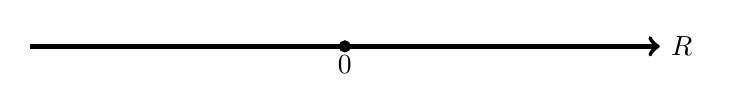
\begin{tikzpicture}
    \draw[->,ultra thick] (-4,0)--(4,0) node[right]{$\mathbb R$};
    \filldraw[black] (0,0) circle (2pt);
    \node[below] at (0,0) {0};

    \end{tikzpicture}
    \caption{A reta real.}
\end{figure}

Lembremos que $\mathbb R^2$ é o conjunto de todos os pares ordenados $(x, y)$, onde $x, y \in \mathbb R$.
Em símbolos:
\begin{equation*}
    \mathbb R^2 = \{(x, y) : x, y \in \mathbb R\}.
\end{equation*}

Em analogia à representação de $\mathbb R$ como uma reta, podemos visualizar $\mathbb R^2$ como o conjunto dos pontos de um plano Cartesiano.
\begin{figure}[ht]
    \centering
    \begin{tikzpicture}
    \draw[->,ultra thick] (-4,0)--(4,0) node[right]{$x$};
    \draw[->,ultra thick] (0,-4)--(0,4) node[above]{$y$};
    % Ponto (2,3)
    \filldraw[black] (2,3) circle (2pt);
    \node[above right] at (2,3) {$(2,3)$};
    \draw[dotted] (2,0) -- (2,3);
    \draw[dotted] (0,3) -- (2,3);
    \draw (2,0.1) -- (2,-0.1);
    \node[below] at (2,0) {2};
    \draw (0.1,3) -- (-0.1,3);
    \node[left] at (0,3) {3};
    \node[below left] at (0,0) {0};

    \end{tikzpicture}
    \caption{O plano Cartesiano.}
\end{figure}

Por sua vez, o conjunto de todas as triplas ordenadas de números reais é denotado por $\mathbb R^3$.
Em símbolos:
\begin{equation*}
    \mathbb R^3 = \{(x, y, z) : x, y, z \in \mathbb R\}.
\end{equation*}

Seguindo o padrão já comentado, podemos visualizar $\mathbb R^3$ como o conjunto dos pontos do espaço tridimensional.

\begin{figure}[ht]
    \centering
    \tdplotsetmaincoords{70}{110}
    \begin{tikzpicture}[tdplot_main_coords]
    % Eixos
    \draw[->,ultra thick] (-4,0,0)--(4,0,0) node[right]{$x$};
    \draw[->,ultra thick] (0,-4,0)--(0,4,0) node[above]{$y$};
    \draw[->,ultra thick] (0,0,-4)--(0,0,4) node[above]{$z$};
    % Ponto (2,3,1)
    \filldraw[black] (2,3,1) circle (2pt);
    \node[above right] at (2,3,1) {$(2,3,1)$};
    % Linhas pontilhadas
    \draw[dotted] (2,0,0) -- (2,3,0) -- (2,3,1);
    \draw[dotted] (0,3,0) -- (2,3,0);
    \draw[dotted] (2,0,0) -- (2,0,1) -- (2,3,1);
    \draw[dotted] (0,0,1) -- (2,0,1);
    % Marcas nos eixos
    \draw (2,0.1,0) -- (2,-0.1,0);
    \node[below] at (2,0,0) {2};
    \draw (0.1,3,0) -- (-0.1,3,0);
    \node[left] at (0,3,0) {3};
    \draw (0.1,0,1) -- (-0.1,0,1);
    \node[left] at (0,0,1) {1};
    \node[below left] at (0,0,0) {0};

    \end{tikzpicture}
    \caption{O espaço tridimensional.}
\end{figure}

No geral, para $n\geq 4$, o conjunto $\mathbb R^n$ é definido como o conjunto de todas as $n$-tuplas ordenadas de números reais:
\begin{equation*}
    \mathbb R^n = \{(x_1, \ldots, x_n) : x_1, \ldots, x_n \in \mathbb R\}.
\end{equation*}

Tal conjunto não possui uma representação gráfica simples a estilo dos anteriores.
Porém, a teoria desenvolvida para $\mathbb R^n$ é uma extensão natural da teoria desenvolvida para $\mathbb R$ e $\mathbb R^2$, e possui amplas aplicações práticas e teóricas.

Elementos de $\mathbb R^n$ serão frequentemente chamados de \emph{pontos} ou \emph{vetores}.
Portanto, neste texto, pontos e vetores serão os mesmos objetos matemáticos, e tais palavras podem ser usadas indistintamente.
A palavra \emph{ponto} será usualmente utilizada em situações em que se faz referência a posições no espaço, enquanto a palavra \emph{vetor} é mais utilizada em situações em que pensamos na direção, sentido e comprimento determinados pelo ponto com relação à origem $0=(0, \ldots, 0)$.